\section{IIR Digital Filter Design\buch{Chapter 11}}
\subsection{Bilinear Transformation\buchSeite{563-565}}
Designflow:
\begin{center}
\begin{tikzpicture}[
	node distance=3cm,
	block/.style={text width=2.5cm,text centered
	}]
\node[draw, block] (dfs) {digital filter specifications};
\node[draw, block, right=of dfs] (afs) {analog filter specifications};
\node[draw, block, below=1cm of dfs] (df) {digital filter \\ $H(z)$};
\node[draw, block, below=1cm of afs] (af) {analog filter \\ $H_a(s)$};
\node[draw, block, below=0cm of afs, xshift=3cm, rounded corners] (afdm) {analog filter design method};

\draw[-stealth, thick] (dfs) -- (afs) 
	node[block, midway, above] {bilinear \\ transformation}
	node[block, midway, below] {$\Omega = g(\omega)$};
\draw[-stealth, thick] (dfs) -- (df);

\draw[-stealth, thick] (af) -- (df) 
	node[block, midway, above] {bilinear \\ transformation}
	node[block, midway, below] {$s = f(z)$};
\draw[-stealth, thick] (afs) -- (af);

\draw[-stealth, thick] (afdm) -- +(-3,0);
\end{tikzpicture}
\end{center}
Maps from z-plane to the s-plane (from the analog frequency to the digital
frequency)

\begin{tabularx}{0.8\textwidth}{|l|X|X|}
	\hline
	\textbf{Filter} & \textbf{bilinear transformation} & \textbf{frequency map}
	\\ \hline
	lowpass & 
	$s = f(z) = \frac{1 - z^{-1}}{1 + z^{-1}}$ &
	$ \Omega = g(\omega) = \tan(\frac{\omega}{2})$
	\\ \hline
	highpass & 
	$s = f(z) = \frac{1 + z^{-1}}{1 - z^{-1}}$ &
	$ \Omega = g(\omega) = - \cot(\frac{\omega}{2})$
	\\ \hline
	bandpass & 
	$s = f(z) = \frac{1 - 2cz^{-1} +z^{-2}}{1 - z^{-2}}$ &
	$ \Omega = g(\omega) = \frac{c - \cos(\omega)}{\sin(\omega)}$
	\\ \hline
	bandstop & 
	$s = f(z) = \frac{1 - z^{-2}}{1 - 2cz^{-1} + z^{-2}}$ &
	$ \Omega = g(\omega) = \frac{\sin(\omega)}{\cos(\omega) - c}$ 
	\\ \hline
\end{tabularx}

\subsection{First-Order LP/HP, Second-Order Peaking an Notching Filters\buchSeite{566-581}}

\paragraph{Definitions}~\\
\begin{tabular}{|l|l|l|}
	\hline
	cutoff/center frequency & $f_c$ &
	\\ \hline
	sampling rate & $f_s$ &
	\\ \hline
	bandwith & $\Delta f$ & Peaking/Notching filter only
	\\ \hline
	digital cutoff/center frequency & $\omega_c$ & $ = \frac{2\pi f_c}{f_s}$ \qquad (usually at 3dB-point)
	\\ \hline
	drop in dB at $f_c$ & $A_c$ & $= -10\log_{10}(G_c^2) = -20\log_{10}(G_c)$ \qquad (usually 3dB)
	\\ \hline
	drop factor & $G_c$ & $=10^{-A_c/20} \qquad \longrightarrow $ If $A_c = 3$dB $\rightarrow G_c^2 = 1/2$
	\\ \hline
\end{tabular}
\vfill
\begin{tabularx}{\textwidth}{|X|l|l|l|l|l|}
	\hline
	\textbf{filter} & $H(z) = $ & $H_a(s) = $ & $\alpha = $ & $a=$ & $b=$
	\\ \hline
	low-pass	&
	$b\frac{1 + z^{-1}}{1 - a z^{-1}}$ &
	$\frac{\alpha}{s + \alpha}$	&
	$ \frac{G_c}{\sqrt{1-G_c^2}}\tan\left(\frac{\omega_c}{2}\right)
	= \tan\left(\frac{\omega_c}{2}\right)\vert_{G_c^2 = \frac{1}{2}}$&
	$\frac{1 - \alpha}{1 + \alpha}$ &
	$\frac{\alpha}{1 + \alpha} = \frac{1 - a}{2}$	
	\\ \hline
	high-pass &
	$b\frac{1 - z^{-1}}{1 - a z^{-1}}$ &
	$\frac{s}{s + \alpha}$ &
	$\frac{\sqrt{1-G_c^2}}{G_c}\tan\left(\frac{\omega_c}{2}\right)
	=\tan\left(\frac{\omega_c}{2}\right)\vert_{G_c^2 = \frac{1}{2}}$&
	$\frac{1-\alpha}{1+\alpha}$&
	$\frac{1}{1+\alpha} = \frac{1 + a}{2}$
	\\ \hline
	notch &
	$b\frac{1-2\cos(\omega_0) z^{-1} + z^{-2}}{1 -2b \cos(\omega_o) z^{-1} + (2b-1)z^{-2}}$&
	$\frac{s^2 + \Omega_0^2}{s^2+\alpha s + \Omega_0^2}$&
	$\frac{\sqrt{1-G_B^2}}{G_B}(1+\Omega_0^2)\tan\left(\frac{\Delta\omega}{2}\right)$&
	--&
	$\frac{1}{1+\frac{\sqrt{1-G_B^2}}{G_B}\tan\left(\frac{\Delta\omega}{2}\right)}$
	\\ \hline
	peak &
	$(1-b)\frac{1-z^{-2}}{1-2b\cos(\omega_0)z^{-1} + (2b-1)z^{-2}}$&
	$\frac{\alpha s}{s^2 + \alpha s + \Omega_0^2}$&
	$\frac{G_B}{\sqrt{1-G_B^2}}(1+\Omega_0^2)\tan\left(\frac{\Delta\omega}{2}\right)$&
	--&
	$\frac{1}{1+\frac{G_B}{\sqrt{1-G_B^2}}\tan\left(\frac{\Delta\omega}{2}\right)}$
	\\ \hline
\end{tabularx}

\paragraph{Designflow} ~\\
\begin{enumerate}
	\item Given the cutoff frequency $\omega_c$ and the corresponding gain $A_c$ in dB, compute $G_c$.
	\item Compute the analog parameter $\alpha$
	\item Compute the digital filter coefficients $\{a,b\}$.
\end{enumerate}


\subsection{Higher Order Filters\buchSeite{592-631}}
The quantities $\{\epsilon_{pass}, \epsilon_{stop}\}$ control the depths of the passband and stopband.
They can be written in the equivalent forms:
\begin{align*}
	\epsilon_{pass} &= \sqrt{10^{A_{pass}/10} - 1} & \Longleftrightarrow &&
	A_{pass}&= 10\log_{10}(1 + \epsilon_{pass}^2) \\
	\epsilon_{stop} &= \sqrt{10^{A_{stop}/10} - 1} & \Longleftrightarrow &&
	A_{stop}&= 10\log_{10}(1 + \epsilon_{stop}^2)
\end{align*}

The specifications of the equivalent analog filter are $\{\Omega_{pass}, \Omega_{stop}, A_{pass}, A_{stop} \}$, or, $\{\Omega_{pass}, \Omega_{stop}, \epsilon_{pass}, \epsilon_{stop} \}$, where the analog frequencies are obtained by prewraping the digital frequencies.
\begin{align*}
	\Omega_{pass} &= \tan\left(\frac{\omega_{pass}}{2}\right) & 
	\Omega_{stop} &= \tan\left(\frac{\omega_{stop}}{2}\right) \\
	\omega_{pass} &= \frac{2\pi f_{pass}}{f_s} &
	\omega_{stop} &= \frac{2\pi f_{stop}}{f_s} 
\end{align*}

\subsubsection{Analog Lowpass Butterworth Filters\buchSeite{594-599}}
Analog lowpass Butterworth filters are characterized by just two parameters:
filter order $N$ and the 3-dB normalization frequency $\Omega_0$.
\[
	\left|H(\Omega)\right|^2 =
		\frac{1}{1 + \left(\frac{\Omega}{\Omega_0}\right)^{2N}}
\]

With the given information, we can calculate the two parameters:
\begin{align*}
	N_{exact} &= \frac{
			\ln(\epsilon_{stop} / \epsilon_{pass})
		}{
			\ln(\Omega_{stop} / \Omega_{pass})
		}
	= \frac{\ln(e)}{\ln(w)} &	
	e &= \frac{\epsilon_{stop}}{\epsilon_{pass}}
	   = \sqrt{\frac{10^{A_{stop}/10} -1}{10^{A_{pass}/10} -1}}&
	w &= \frac{\Omega_{stop}}{\Omega_{pass}}&	
\end{align*}

$N$ must be an integer, we round $N_{exact}$ up to the nearest integer: $N = \lceil N_{exact} \rceil$

\[
	\Omega_0 = \frac{
			\Omega_{pass}
		}{
			\left(10^{A_{pass}/10}-1\right)^{1/2N}
		} = \frac{
			\Omega_{pass}
		}{
			\epsilon_{pass}^{1/N}
		}
\]

Of course , $\Omega_0$ can be calculated in terms of the stopband. Then the
passband attenuation will be a bit smaller than necessary. 

\paragraph{Spectral factorization}
The amplitude response $\left|H(\Omega)\right|^2$ now has to be transformed
into a transfer function $H(\Omega)$. With $s = j \Omega$, the fact that
$\left|H(\Omega)\right|^2 = H(\Omega) H(\Omega)^*$ and setting 
$H(s) = \frac{1}{D(s)}$, we have
\begin{equation*}
	D(s) D(-s)^* = 1 + (-1)^N \left( \frac{s}{\Omega_0} \right)^{2N}
\end{equation*}

\vspace{1em}

\begin{multicols}{2}
	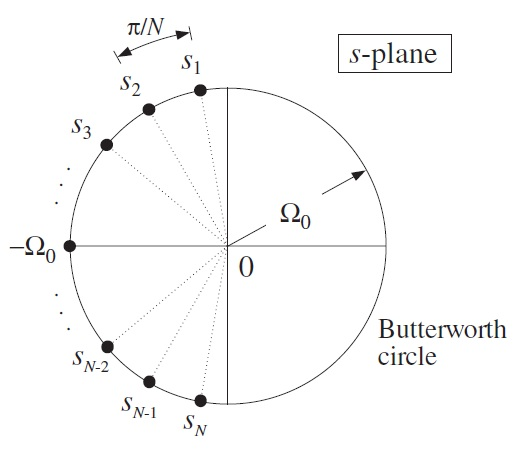
\includegraphics[width=7cm]{images/IIR_ButterworthCircle.jpg}
\vfill
\columnbreak

	To find a $H(s)$ that is causal and stable, we have to find all the roots
	in the left hand side of the s-plane of the following polynomial:
	\begin{equation*}
		1 + (-1)^N \left(\frac{s}{\Omega_0}\right)^{2N} = 0 \qquad \Rightarrow \qquad s^{2N} = (-1)^{N-1} \Omega_0^{2N}
	\end{equation*}
	
	The $2N$ roots are equally spaced on a circle in the s-plane with the radius
	of $\Omega_0$. 
	\begin{equation*}
		s_i = \Omega_0 e^{j \theta_i} \:, \quad \theta_i = \frac{\pi}{2N} (N - 1 + 2i) \:, \quad  i = 1,2,\ldots,2N
	\end{equation*}
\end{multicols}

If $N$ is even $(N = 2K)$, there are exactly $K$ conjugate complex root pairs.
If $N$ is odd $(N = 2K+1)$, there are $k$ conjugate complex root pairs and one
single root at $s = -\Omega_0$. The conjugate complex pairs can be written as
second order section, allowing to write $H(s)$ as \\

\begin{align*}
	H(s) &= H_0(s) H_1(s) H_2(s) \ldots H_K(s) \qquad \text{where} \qquad
	\begin{array}{ll}
		H_0(s) & = \begin{cases}
			1\:, & \text{if} \quad N = 2K \\
			\frac{1}{1 + \frac{s}{\Omega_0}} \:, & \text{if} \quad N = 2K+1
			\end{cases} \\
		H_i(s) &= \frac{1}{1 - 2 \frac{s}{\Omega_0} \cos\theta_i + \frac{s^2}{\Omega_0^2}} \:,\quad i=1,2,\ldots,K
	\end{array}
\end{align*}

A list of Butterworth polynomials can be found in appendix \ref{app:Butterworth}.

\paragraph{Design steps}
\begin{enumerate}
	\item Calculate the digital frequencies $\{\omega_{pass}, \omega_{stop}\}$ 
	and the corresponding prewarped version $\{\Omega_{pass}, \Omega_{stop}\}$.
	\item Calculate the order-$N$ and the 3-dB frequency $\Omega_0$ of the
	 equivalent analog Butterworth filter based on the transformed specifications
	 $\{\Omega_{pass}, \Omega_{stop}, A_{pass}, A_{stop} \}$
	\item Calculate the coefficients for all second-order sections and the transfer function.
\end{enumerate}

\subsubsection{Digital Lowpass Filters\buchSeite{599ff}}
As before, the analog lowpass filter must be transformed into a digital
filter using the bilinear transform

\begin{equation*}
	H_i(z) = \left.\frac{1}{1 - 2 \frac{s}{\Omega_0}\cos\theta_i + \frac{s^2}{\Omega_0^2}}\right|_{s = \frac{1-u^{-1}}{1+z^{-1}}} = 
	\frac{G_i (1+z^{-1})^2}{1 + a_{i1}z^{-1} + a_{i2}z^{-2}}
\end{equation*}

where the filter coefficients $G_i, a_{i1}, a_{i2}$ are easily found to be

\begin{equation*}
	G_i = \frac{\Omega_0^2}{1 - 2 \Omega_0 \cos\theta_i + \Omega_0^2} \qquad
	a_{i1} = \frac{2(\Omega_0^2 - 1)}{1 - 2 \Omega_0 \cos\theta_i + \Omega_0^2} \qquad
	a_{i2} = \frac{1 + 2 \Omega_0 \cos\theta_i + \Omega_0^2}{1 - 2 \Omega_0 \cos\theta_i + \Omega_0^2}
\end{equation*}

If $N$ is odd, there is of course a first-order section

\begin{equation*}
	H_0(z) = \left.\frac{1}{1+\frac{s}{\Omega_0}}\right|_{s = \frac{1-z^{-1}}{1+z^{-1}}}
	= \frac{G_0 (1+z^{-1})}{1 + a_{01} z^{-1}}
	\qquad \text{with} \qquad
	G_0 = \frac{\Omega_0}{\Omega_0 + 1} \:,\quad 
	a_{01}=\frac{\Omega_0 - 1}{\Omega_0 + 1}
\end{equation*}

This results in the overall digital transfer function 
$H(z) = H_0(z) H_1(z) H_2(z) \ldots H_K(z)$. The 3dB frequency
$f_0$ in Hz is related to the Butterworth parameter $\Omega_0$ over the
bilinear transform:
\begin{equation*}
	f_0 = \frac{f_s}{\pi} \arctan(\Omega_0)
\end{equation*}

\subsubsection{Digital Highpass Filters\buchSeite{603ff}}
The highpass version of the bilinear transform is used to map the given
highpass specifications onto equivalent analog lowpass specifications. \\

For a highpass filter, the passband and stopband frequencies are calulated
by

\begin{align*}
	\Omega_{pass} &= \cot \left( \frac{\omega_{pass}}{2} \right)
	= \cot\left( \frac{\pi f_{pass}}{f_s} \right) \\
	\Omega_{pass} &= \cot\left(\frac{\omega_{stop}}{2}\right)
	= \cot\left(\frac{\pi f_{stop}}{f_s}\right)
\end{align*}

The highpass bilinear transform is then used to find $H(z)$
\begin{align*}
	H_i(z) &= \frac{G_i (1-z^{-1})^2}{1 + a_{i1} z^{-1}+a_{i2}z^{-2}} \\
	\text{where} \\
	G_i = \frac{\Omega_0^2}{1-2\Omega_0\cos\theta_i + \Omega_0^2} \qquad
	a_{i1} &= -\frac{2(\Omega_0^2-1)}{1-2\Omega_0\cos\theta_i + \Omega_0^2} \qquad
	a_{i2} = \frac{1 + 2\Omega_0\cos\theta_i + \Omega_0^2}{1-2\Omega_0\cos\theta_i + \Omega_0^2}
\end{align*}

Again, if $N$ is odd, then there is a first-order section
\begin{equation*}
	H_0(z) = \frac{G_0(1-z^{-1})}{1 + a_{01} z^{-1}} \qquad \text{where} \quad
	G_0 = \frac{\Omega_0}{\Omega_0 + 1} \:,\quad 
	a_{01} = -\frac{\Omega_0 - 1}{\Omega_0 + 1}
\end{equation*}

The 3dB frequency $f_0$ of the highpass filter can then be calculated as
\begin{equation*}
	f_0 = \frac{f_s}{\pi} \arctan\left(\frac{1}{\Omega_0}\right)
\end{equation*}

Note the similarities and differences between the highpass and the lowpass
case: The coefficients $G_i$ and $a_{i2}$ are the same, but $a_{i1}$ has
reverse sign. The numerator of the second order sections is now $(1-z^{-1})^2$
instead of $(1+z^{-1})^2$, resulting in a zero at $z=1$ or $\omega=0$.

\subsubsection{Digital Bandpass Filters\buchSeite{606ff}}
The bandpass filter design works similarly. This design will result in the
same attenuation in both stopbands. Hence one must focus on the stopband
with the more stringent specification. \\

The bandpass specifications are mapped onto the entire passband 
$[-\Omega_{pass}\:,\:\Omega_{pass}]$ of the analog filter by

\begin{equation*}
		\Omega = \frac{c - \cos\omega}{\sin\omega} \qquad \text{where} \qquad
		c = \frac{\sin\left(\omega_{pa}+\omega_{pb}\right)}
		{\sin\omega_{pa}+\sin\omega_{pb}}
\end{equation*}

Note that $c=\cos\omega_c$ where $\omega_c$ can be thought of as the center
frequency of the bandpass filter. In general $\omega_c$ is \emph{not} exactly
the the center of the passband! \\

This results in
\begin{equation*}
	\Omega_{pass} = \left| \frac{c - \cos\omega_{pb}}{\sin\omega_{pb}} \right|
	\qquad \text{and} \qquad
	\Omega_{stop} = \min\left( |\Omega_{sa}|\:,\:|\Omega_{sb}| \right)
	\quad \text{with} \quad
	\Omega_{sa} = \frac{c-\cos\omega_{sa}}{\sin\omega_{sa}}\:, \quad
	\Omega_{sb} = \frac{c-\cos\omega_{sb}}{\sin\omega_{sb}}
\end{equation*}

Again, $H_i(z)$ and, if $N$ is odd also $H_0(z)$ are calculated as
\begin{align*}
	H_i(z) &= \frac{G_i (1-z^{-2})^2}{1 + a_{i1}z^{-1} + a_{i2}z^{-2} + a_{i3}z^{-3} + a{i4}z^{-4}}
	\qquad \text{where} \quad
	G_i = \frac{\Omega_0^2}{1-2\Omega_0\cos\theta_i+\Omega_0^2} \\
	a_{i1} &= \frac{4c(\Omega_0\cos\theta_i-1)}{1-2\Omega_0\cos\theta_i+\Omega_0^2} \qquad
	a_{i2} = \frac{2(2c^2+1-\Omega_0^2)}{1-2\Omega_0\cos\theta_i+\Omega_0^2} \\
	a_{i3} &= -\frac{4c(\Omega_0\cos\theta_i+1)}{1-2\Omega_0\cos\theta_i+\Omega_0^2} \qquad
	a_{i4} = \frac{1+2\Omega_0\cos\theta_i+\Omega_0^2}{1-2\Omega_0\cos\theta_i+\Omega_0^2} \\
	\text{and} \\
	H_0(z) &= \frac{G_0(1-z^{-2})}{1+a_{01}z^{-1}+a_{02}z^{-2}} \qquad \text{where} \\
	G_0 &= \frac{\Omega_0}{1+\Omega_0} \:,\qquad 
	a_{01} = -\frac{2c}{1+\Omega_0} \:,\qquad 
	a_{02} = \frac{1-\Omega_0}{1+\Omega_0}
\end{align*}

Each filter section has zeros at $z=\pm 1$, i.e. $\omega=0$ and $\omega=\pi$. 
The left and the right 3dB frequencies $\omega_{0a}$ and $\omega_{0b}$ can be
calculated by
\begin{equation*}
	\tan\left(\frac{\omega_{0a}}{2}\right) = \frac{\sqrt{\Omega_0^2+1-c^2}-\Omega_0}{1+c}
	\qquad \text{and} \qquad
	\tan\left(\frac{\omega_{0b}}{2}\right) = \frac{\sqrt{\Omega_0^2+1-c^2}+\Omega_0}{1+c}
\end{equation*}

\subsubsection{Digital Bandstop Filters\buchSeite{611ff}}
The design of digital bandstop filters is similar to that of digital
bandpass filters.

\begin{align*}
	c &= \frac{\sin(\omega_{pa}+\omega_{pb})}{\sin\omega_{pa}+\sin\omega_{pb}}
	\:,\qquad
	\Omega_{pass} = \left| \frac{\sin\omega_{pb}}{\cos\omega_{pb}-c} \right| \\
	\Omega_{stop} &= \min\left(|\Omega_{sa}|,|\Omega_{sb}|\right)
	\qquad \text{where} \quad
	\Omega_{sa} = \frac{\sin\omega_{sa}}{\cos\omega_{sa}-c}\:,\quad
	\Omega_{sb} = \frac{\sin\omega_{sb}}{\cos\omega_{sb}-c}
\end{align*}

The bilinear transform of the second order sections is then
\begin{align*}
	H_i(z) &= \frac{G_i(1-2cz^{-1}+z^{-2})^2}{1+a_{i1}z^{-1}+a_{i2}z^{-2}+a_{i3}z^{-3}+a_{i4}z^{-4}}
	\qquad \text{where} \quad
	G_i = \frac{\Omega_0^2}{1-2\Omega_0\cos\theta_i+\Omega_0^2} \\
	a_{i1} &= \frac{4c\Omega_0(\cos\theta_i-\Omega_0)}{1-2\Omega_0\cos\theta_i+\Omega_0^2} \qquad
	a_{i2} = \frac{2(2c^2\Omega_0^2+\Omega_0^2-1)}{1-2\Omega_0\cos\theta_i+\Omega_0^2} \\
	a_{i3} &= \frac{4c\Omega_0(\cos\theta_i+\Omega_0)}{1-2\Omega_0\cos\theta_i+\Omega_0^2} \qquad
	a_{i4} = \frac{1+2\Omega_0\cos\theta_i+\Omega_0^2}{1-2\Omega_0\cos\theta_i+\Omega_0^2} \\
	\text{and} \\
	H_0(z) &= \frac{g_0(1-2cz^{-1}+z^{-2})}{1+a_{01}z^{-1}+a_{02}z^{-2}} \qquad \text{where} \\
	G_0 &= \frac{\Omega_0}{1+\Omega_0}\:,\qquad
	a_{01} = -\frac{2c\Omega_0}{1+\Omega_0} \:,\qquad
	a_{02} = -\frac{1-\Omega_0}{1+\Omega_0}
\end{align*}

Each second order section has zeros at $\omega = \pm \omega_c$,  which makes
sense for a bandstop filter. The 3dB frequencies are now
\begin{equation*}
	\tan\left(\frac{\omega_{0a}}{2}\right) = \frac{\sqrt{1+\Omega_0^2(1-c^2)}-1}{\Omega_0(1+c)}
	\tan\left(\frac{\omega_{0b}}{2}\right) = \frac{\sqrt{1+\Omega_0^2(1-c^2)}+1}{\Omega_0(1+c)}
\end{equation*}
